% ── 4. Results and Discussion ─────────────────────────────────────────────────
\section{Results and Discussion}
\label{sec:results}

\subsection{Evaluation Protocol}
\label{sec:eval}

We adopt PathRAG's~\cite{chen2025pathrag} five-dimension head-to-head
evaluation criteria extended to a multi-judge protocol.
Each GRASP-RAG answer is compared against a baseline answer by three
independent judges: GPT-4o-mini, Claude Haiku, and Gemini~2.0~Flash.
Each judge runs twice per comparison---\emph{forward} (GRASP-RAG as Answer~1)
and \emph{reversed} (GRASP-RAG as Answer~2)---to control for position bias;
a win is counted only when both orderings agree on the preferred system.
Final outcomes per dimension (Comprehensiveness, Diversity, Logicality,
Coherence, Relevance) are determined by majority vote across the three judges.
When two or more judges mark a dimension as ``Cannot Evaluate'' because both
answers fail to address the question, the dimension is recorded as
\textbf{Undefined} and excluded from the win/loss denominator.
Win rate is the fraction of (question, dimension) pairs where GRASP-RAG wins,
excluding Undefined decisions.

Two limitations of this protocol are worth stating upfront.
GPT-4o-mini serves as both the answer-generation backbone and one of the three
judges; self-preference effects are not independently quantified.
Because all four systems (GRASP-RAG, NaiveRAG, LightRAG, PathRAG) use
GPT-4o-mini for generation, however, self-preference cannot systematically
favour GRASP-RAG over baselines in absolute terms---the concern is rather
that GPT-4o-mini-as-judge may prefer certain answer structures, a confound
the current protocol does not control.
Second, each per-cell result is a point estimate over 100--405 questions, so
numerical differences smaller than a few percentage points should not be
over-interpreted.

\subsection{Experiment 1: Win Rate on UltraDomain}
\label{sec:exp1}

The goal of Experiment~1 is to measure whether GRASP-RAG's answers are
factually closer to expert-written references than baseline answers.
We use the UltraDomain benchmark~\cite{ding2024ultradomain} questions, which
carry reference answers written by domain experts, and evaluate with a
reference-anchored judge that asks which answer is \emph{more accurate relative
to the reference}---not which the judge prefers in isolation.
This is a harder and more externally valid comparison than pairwise preference
without a reference.
UltraDomain's reference answers are provided by the benchmark's creators and
described as domain-expert-authored; we have not independently verified the
credentials of the authors or the factual accuracy of the references.

Table~\ref{tab:winrate} reports GRASP-RAG's win rate against each baseline,
averaged across all five evaluation dimensions.
Questions per domain: 100 (Agriculture), 100 (CS), 405 (Legal), 180 (Health);
differing sample sizes reflect the question sets available per domain and
affect the statistical reliability of per-domain comparisons.
Legal had 426 independently labelled questions in total; 21 lacked evaluation results
and are excluded from win-rate calculations but included in the classifier
confusion matrix (Figure~\ref{fig:confusion}), which accounts for the
difference between the 806-question matrix and the 785-question per-type
Table~\ref{tab:winrate_bytype}.
The Undef.\% column shows the fraction of dimension decisions where both
systems failed simultaneously (vs.\ LightRAG; other baselines are similar).

\begin{table}[t]
\caption{GRASP-RAG win rate (\%) vs.\ each baseline, averaged across all five
  evaluation dimensions. Win rate\,=\,wins\,/\,(wins\,+\,losses) per
  (question\,$\times$\,dimension) pair; Undefined outcomes excluded.
  Baselines: NaiveRAG = dense-passage retrieval; LightRAG = KG hybrid
  retrieval; PathRAG = flow-based path retrieval.
  Bold = highest win rate per data row.
  Undef.\%$^{\dag}$ = fraction of dimension decisions where both systems
  failed simultaneously; $^{\dag}$reported vs.\ LightRAG---rates vs.\
  other baselines are similar.}
\label{tab:winrate}
\centering
\renewcommand{\arraystretch}{1.15}
\setlength{\tabcolsep}{2.8pt}
\begin{tabular}{lrcccr}
\toprule
\textbf{Domain} & \textbf{n} & \textbf{vs NaiveRAG} & \textbf{vs LightRAG} &
  \textbf{vs PathRAG} & \textbf{Undef.\%}$^{\dag}$ \\
\midrule
Agriculture & 100 &          65.2 &          77.7 & \textbf{79.7} & 23.8 \\
CS          & 100 &          83.2 & \textbf{86.3} &          83.7 & 17.0 \\
Legal       & 405 &          39.5 &          52.5 & \textbf{74.2} & 25.1 \\
Health      & 180 &          65.4 &          77.0 & \textbf{81.3} & 28.1 \\
\midrule
\textbf{Average} & --- & 63.3 & 73.4 & \textbf{79.7} & 23.5 \\
\bottomrule
\end{tabular}
\end{table}

The clearest pattern in Table~\ref{tab:winrate} is that GRASP-RAG's most
consistent advantage is against \emph{PathRAG}, the strongest baseline.
The average win rate of 79.7\% against PathRAG holds across all four domains
and is the most stable number in the table; it remains above 74\% in every
domain, reaching a minimum of 74.2\% in Legal where GRASP-RAG struggles
against the other baselines.
Against LightRAG the story is also positive---73.4\% average---though the
Legal result (52.5\%) is close to parity and the Undefined fraction is
substantial everywhere (17--28\%), meaning a significant share of questions
causes both systems to produce uninformative answers.

The Legal domain against NaiveRAG (39.5\%) is the one result where GRASP-RAG
clearly loses, and the cause is two-fold.
Error analysis shows that 53.8\% of losing Legal questions carry a
classifier--reference type mismatch, versus 29.1\% of winning questions: routing
errors concentrate in the loss column.
The most common error is routing a single-entity question through the bridge
path, adding multi-hop traversal where an ego-graph would have been
appropriate.
But misclassification is not the complete explanation.
Oracle bridge questions in Legal (32 questions, classified correctly 84.4\%
of the time) still lose on Relevance at 7.7\% against NaiveRAG.
The Legal KG does not help any graph traversal motif against NaiveRAG's chunk
retrieval.
UltraDomain Legal reference answers emphasise broad coverage of statutory and
regulatory context, and NaiveRAG retrieving many passages from the
KG-extracted content matches that coverage pattern better than a graph
traversal anchored on specific named entities, regardless of which motif is
selected.

\paragraph{On Undefined outcomes.}
The Undefined fraction (17--28\%) is high enough to affect interpretation,
and its distribution across query types is not random.
Broad queries produce Undefined rates 5--18 percentage points above the
per-domain average against NaiveRAG and LightRAG: when both systems fall back
to general keyword or passage retrieval on a thematic question, neither
produces a clearly better answer and judges mark both as unevaluable.
Bridge queries show the opposite pattern against NaiveRAG and LightRAG
(Undefined below average), because GRASP-RAG traverses a specific hop chain
while the baselines do keyword matching---the answers are structurally
different and easy to compare.
Against PathRAG, however, bridge query Undefined rates are above average:
PathRAG's flow-based pruning discards low-frequency edges, so both systems
tend to miss the same specific connections and fail simultaneously.
Undefined fractions are similar across all three baselines (no baseline
systematically avoids shared-failure outcomes), so all three win rates are
comparably affected.

% ── Win-rate bar chart ────────────────────────────────────────────────────────
\begin{figure}[t]
\centering
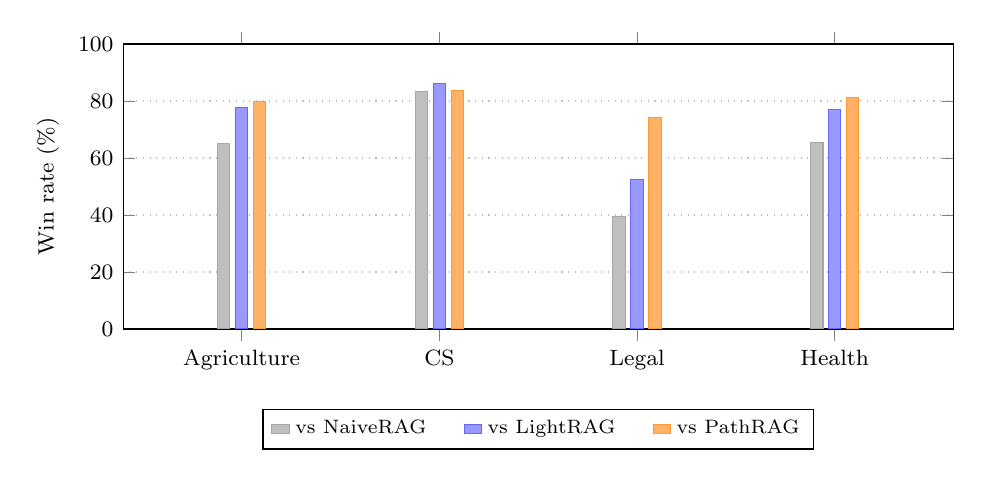
\begin{tikzpicture}
\begin{axis}[
  ybar,
  bar width=4.5pt,
  width=\columnwidth,
  height=5.2cm,
  ymajorgrids=true,
  grid style={dotted,gray!50},
  ylabel={Win rate (\%)},
  ymin=0, ymax=100,
  xtick={0,1,2,3},
  xticklabels={Agriculture, CS, Legal, Health},
  x tick label style={font=\footnotesize},
  y tick label style={font=\footnotesize},
  ylabel style={font=\footnotesize},
  legend style={font=\scriptsize, at={(0.5,-0.28)}, anchor=north,
                legend columns=3, /tikz/every even column/.append style={column sep=0.4cm}},
  legend image code/.code={\draw[#1] (0cm,-0.06cm) rectangle (0.22cm,0.06cm);},
  enlarge x limits=0.2,
]
% vs NaiveRAG
\addplot[fill=gray!50,draw=gray!70] coordinates {(0,65.2)(1,83.2)(2,39.5)(3,65.4)};
% vs LightRAG
\addplot[fill=blue!40,draw=blue!60] coordinates {(0,77.7)(1,86.3)(2,52.5)(3,77.0)};
% vs PathRAG
\addplot[fill=orange!60,draw=orange!80] coordinates {(0,79.7)(1,83.7)(2,74.2)(3,81.3)};
\legend{vs NaiveRAG, vs LightRAG, vs PathRAG}
\end{axis}
\end{tikzpicture}
\caption{GRASP-RAG win rate (\%) by domain and baseline (Experiment~1,
  reference-anchored). The advantage against PathRAG is the most consistent
  across domains; Legal shows a sharp split between baselines.}
\label{fig:winrate_chart}
\end{figure}

\subsection{Experiment 2: Classifier Accuracy and Per-Type Win Rate}
\label{sec:exp2}

Experiment~1 shows that GRASP-RAG wins overall, but it does not tell us
whether the routing machinery is actually working---it is possible the win
comes from the topology-aware context structuring alone, independent of which
motif was selected.
We use two distinct metrics: \emph{classifier accuracy} measures how often the
system's predicted query type matches the independent GPT-4o label; \emph{win
rate} measures how often GRASP-RAG's answer beats a baseline's answer on a
given dimension (regardless of whether the query was correctly typed).
Experiment~2 examines two related questions: how accurately does the
classifier identify query types, and does GRASP-RAG win across types even
when classification is imperfect?

\paragraph{Classifier accuracy.}
We compare GRASP-RAG's automatic type assignments against independently
produced labels from GPT-4o (a stronger labeling model than the GPT-4o-mini
classifier); each label was human-verified by the authors before acceptance.
Figure~\ref{fig:confusion} shows the pooled confusion matrix across all four
domains (806 questions total).
Per-domain overall accuracy ranges from 40.0\% (Agriculture) to 72.0\% (CS),
with Legal and Health at 56.3\% and 50.0\% respectively.

\begin{figure}[t]
  \centering
  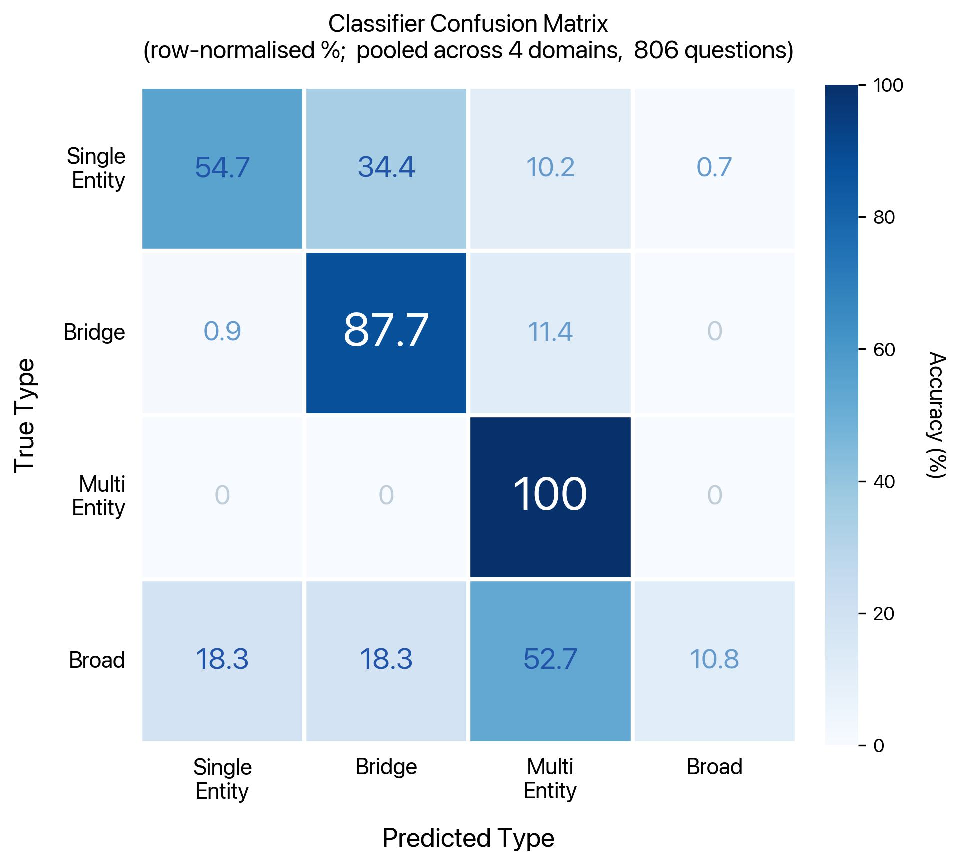
\includegraphics[width=\columnwidth]{confusion_matrix.pdf}
  \caption{Classifier confusion matrix (row-normalised \%), pooled across all
    four UltraDomain domains (806 independently labelled questions, including
    21 Legal questions without evaluation results that are excluded from
    Table~\ref{tab:winrate_bytype}). Bridge is classified reliably
    (87.7\%); broad nearly collapses, with 52.7\% misread as multi-entity.
    Multi-entity shows 100\% on only 9 questions---too small to interpret.}
  \label{fig:confusion}
\end{figure}

Two patterns stand out.
Bridge queries are classified reliably (87.7\% correct pooled): they have
clear structural cues---two named entities and a relational verb.
Broad queries nearly collapse: only 10.8\% are correctly identified, with
52.7\% misread as multi-entity.
This happens because broad questions in the UltraDomain benchmark often
mention domain concepts incidentally, which the classifier interprets as
entity anchors.
Single-entity queries are moderately accurate (54.7\%), with the main
confusion going to bridge (34.4\%)---when a question names a single entity
alongside a domain phrase, the classifier sometimes treats the phrase as a
second anchor.
The multi-entity row shows 100\%, but on only 9 questions across four
domains; that number should not be interpreted as meaningful.

\paragraph{Per-type win rate.}
If classification errors propagate to retrieval errors, we would expect win
rates to drop for the types where the classifier fails.
Table~\ref{tab:winrate_bytype} checks this by grouping Experiment~1's
dimension-level results according to each question's independent label.

\begin{table}[t]
\caption{GRASP-RAG win rate (\%) by independently labeled query type,
  pooled across all four domains (785 evaluated questions; 21 Legal questions
  with independent labels but no evaluation results are excluded; see
  Figure~\ref{fig:confusion} for the full 806-question label set).
  Labels produced by GPT-4o (a stronger labeling model than the GPT-4o-mini
  classifier; each label human-verified by the authors). Win rates stay positive across all types,
  including broad queries where the classifier achieves only 10.8\% accuracy.
  Multi-entity (n\,=\,9) is too small to interpret reliably.}
\label{tab:winrate_bytype}
\centering
\renewcommand{\arraystretch}{1.15}
\setlength{\tabcolsep}{3.5pt}
\begin{tabular}{lcccc}
\toprule
\textbf{Query Type} & \textbf{n} & \textbf{vs NaiveRAG} & \textbf{vs LightRAG} & \textbf{vs PathRAG} \\
\midrule
Single-entity & 569 & 53.4 & 66.2 & 79.9 \\
Bridge        & 114 & 53.6 & 60.1 & 70.9 \\
Multi-entity  & 9   & 60.5 & 72.5 & 74.1 \\
Broad         & 93  & 56.4 & 70.2 & 73.6 \\
\bottomrule
\end{tabular}
\end{table}

The key finding in Table~\ref{tab:winrate_bytype} is that win rates remain
positive for \emph{every} query type against \emph{every} baseline---including
broad queries, where the classifier almost always assigns the wrong label.
This suggests the fallback mechanism limits catastrophic failure when
classification is wrong, though no comparison against a no-fallback baseline
was run to isolate the fallback's independent contribution.
The explanation lies in two mechanisms.
First, when a broad query is misclassified as multi-entity, the Steiner tree
motif runs on the (incorrectly identified) anchor set; the confidence score
\eqref{eq:conf} often falls below the 0.04 threshold on a sparse subgraph,
triggering the fallback to LightRAG hybrid---which is what the broad motif
would have done anyway (we have not logged the fallback trigger rate for
misclassified-broad queries).
Second, even when the wrong motif runs and produces a subgraph, the topology-
aware context structuring may include more specific entity descriptions than a
flat chunk list, which could improve answer quality over baselines that return
generic keyword-matched passages; this has not been isolated experimentally.
This graceful degradation does not make the classification errors
inconsequential---Table~\ref{tab:winrate_bytype} shows that single-entity and
bridge win rates are lower than one would expect from a perfect classifier---
but it does mean the system fails gently rather than catastrophically when
the classifier is wrong.
When grouped by system labels rather than independent labels, win rates follow the
same positive trend across Agriculture, CS, and Health; the exception is
Legal, where questions the classifier routes as bridge achieve only 12--18\%
on Comprehensiveness and Relevance against NaiveRAG, far below the 36--44\%
for questions routed as single-entity.
That bridge-routed group consists predominantly of misclassified single-entity
questions---the dominant classification error in Legal---and matches the
53.8\%-vs-29.1\% mismatch-rate gap described in Section~\ref{sec:exp1}.

\subsection{Discussion}
\label{sec:discussion}

\paragraph{Where the structural advantage is clearest.}
GRASP-RAG's most consistent win is against PathRAG (79.7\% average); one
structural hypothesis is that the motif-routing advantage is most pronounced
against flow-based retrieval.
PathRAG's design assigns reliability scores based on edge traversal frequency:
high-frequency category links (e.g., statute $\to$ provision in Legal,
compound $\to$ metabolic pathway in Health) receive high scores, while
specific bridge edges connecting named entities---which are by definition
low-frequency---may be scored as unreliable and pruned.
GRASP-RAG's bridge motif traverses shortest paths unconditionally, without
filtering by edge frequency.
The Legal domain makes the contrast concrete: GRASP-RAG wins 74.2\% against
PathRAG even while losing to NaiveRAG---a pattern consistent with PathRAG
pruning the low-frequency connections that legal bridge questions target,
though other explanations cannot be ruled out.

\paragraph{Why Legal is hard for everything else.}
Two mechanisms compound in Legal.
Classifier errors concentrate in the loss column: 53.8\% of losing questions
carry a classifier--reference type mismatch, versus 29.1\% of winning questions.
The dominant error is routing a single-entity question through the bridge
path, which introduces extra hops on a question where a direct ego-graph
traversal would have been appropriate.
Domain structure compounds this separately: independently labeled bridge questions in Legal
(correctly classified 84.4\% of the time) still lose on Relevance at 7.7\%
against NaiveRAG.
The Legal KG, built from dense statutory text, is dominated by high-frequency
category links (statute $\to$ provision $\to$ subsection) that connect many
entities but carry little discriminative information per edge.
NaiveRAG retrieving many passages from the same KG-extracted content matches
the broad coverage that Legal reference answers require better than any
graph traversal anchored on named entities.
Improving Legal classification accuracy would reduce losses from misrouted
single-entity questions, but the domain's structural properties mean some gap
against NaiveRAG would likely remain even with perfect routing.

\paragraph{What the per-type pattern tells us.}
Reading Tables~\ref{tab:winrate} and \ref{tab:winrate_bytype} together, the
pattern is: GRASP-RAG outperforms PathRAG most reliably on bridge and single-
entity queries (70.9\% and 79.9\%), and the advantage extends to broad and
multi-entity questions at a lower but still positive level.
The CS domain consistently shows the highest win rates (83--86\% vs.\ all
baselines), which is consistent with CS text having cleaner entity-relation
structure than legal or health text.
Agriculture and Health sit in the middle.
In domains with well-defined entities and explicit relational language, GRASP-
RAG's motif routing gives it a reliable structural advantage; in domains
dominated by procedural or narrative text (Legal), the advantage narrows.

\paragraph{What GRASP-RAG is suited for.}
The results suggest GRASP-RAG is most useful in mixed-question environments
over a structured knowledge graph---that is, applications where a user might
ask definitional, relational, and thematic questions about the same corpus
within the same session.
A fixed-strategy system would do well on the question type it was tuned for
and worse on the others; GRASP-RAG spreads the advantage more evenly by
routing each question to its matched motif.
The classifier's weakness on broad queries (10.8\%) means that corpus-level
thematic questions should ideally be flagged or filtered upstream in a
production system; the per-type win rates show that even on these, the
fallback to LightRAG hybrid is not harmful.

\paragraph{Computational cost.}
GRASP-RAG's cost depends on which execution path is taken.
On the direct path (classifier confident, motif non-broad), each query
requires two GPT-4o-mini calls: one for the classifier and one for answer
generation.
On the cascade path (uncertain classification or broad query type), the
system additionally calls the LLM verifier three times---once per candidate
motif---before generating the answer, for a total of five calls.
NaiveRAG and LightRAG require a single generation call per query; PathRAG is
comparable.
In practice, bridge queries (14\% of the pooled dataset) and correctly
identified single-entity queries (the majority path) take the two-call direct
path; broad queries (12\%) and ambiguous single-entity queries fall through to
cascade or LightRAG hybrid.
The classifier adds one call of latency even on the fast path, which is the
primary cost overhead of the adaptive approach relative to fixed-strategy
baselines.
Latency measurements and per-token cost accounting are left for future
deployment evaluation.

\paragraph{Ablation: context structuring vs.\ graph retrieval.}
To isolate the contribution of topology-aware context serialisation from the
motif's retrieval guarantee, we held routing and graph traversal fixed and
replaced the step-by-step labelled context with a flat serialisation:
entity--description pairs and \texttt{Relation: A\,$\to$\,B | Keywords: \ldots}
triples without hop-chain structure (\textbf{GRASP-RAG-flat}).
Evaluated on Agriculture (100 questions) under the same reference-anchored
multi-judge protocol, the topology-aware variant wins \textbf{62.4\%} of
decided dimension comparisons against GRASP-RAG-flat (Comprehensiveness
62.0\%, Diversity 60.4\%, Logicality 66.0\%, Coherence 63.3\%, Relevance
60.3\%).
The Undefined fraction is high (42--51\%), consistent with both variants
sharing the same retrieval: questions where the retrieved subgraph is
uninformative fail regardless of how context is serialised.
On questions where retrieval provides useful evidence, the step-by-step
topology labels consistently outperform flat serialisation---confirming that
structured context presentation, not just graph traversal, contributes to the
win-rate advantage.

\paragraph{Limitations.}
The context-structuring ablation is evaluated on one domain (Agriculture);
whether the 62.4\% margin replicates on Legal, CS, and Health is left for
future work.
An oracle routing experiment on the same domain---replacing the classifier
with GPT-4o ground-truth labels and VDB-top-$k$ anchor assignment---shows
that GRASP-RAG wins only 42.5\% of decisions against the oracle-routed
variant, meaning perfect routing would recover a further $\sim$15\% of
dimension decisions.
This confirms the classifier is a meaningful bottleneck alongside the
context-structuring contribution.
The anchor assignment in the oracle condition differs from the real system
(VDB candidates vs.\ LLM-extracted named entities), so the gap may partly
reflect anchor quality rather than routing type alone.
Per-judge analysis reveals that GPT-4o-mini, which also generates GRASP-RAG's
answers, awards GRASP-RAG 15--29 percentage points higher win rates against
NaiveRAG and LightRAG than Claude Haiku and Gemini Flash do independently;
the PathRAG comparisons show no such divergence (all three judges agree
within 10\%).
This self-preference inflates the reported NaiveRAG and LightRAG win rates
and means the PathRAG comparison (79.7\% average) is the most credible
result in this evaluation.
The cascade mechanism does not improve substantially over a direct LightRAG
hybrid fallback in the tested settings; we address this in Future Work.
